\documentclass{article}
\usepackage[a4paper, portrait, margin=1.1811in]{geometry}
\usepackage[english]{babel}
\usepackage[utf8]{inputenc}
\usepackage[T1]{fontenc}
\usepackage{helvet}
\usepackage{etoolbox}
\usepackage{graphicx}
\usepackage{titlesec}
\usepackage{caption}
\usepackage{booktabs}
\usepackage{xcolor} 
\usepackage[colorlinks, citecolor=cyan]{hyperref}
\usepackage{caption}
\captionsetup[figure]{name=Figure}
\graphicspath{ {./images/} }
\usepackage{scrextend}
%\usepackage{fancyhdr}
\usepackage{graphicx}
\newcounter{lemma}
\newtheorem{lemma}{Lemma}
\newcounter{theorem}
\newtheorem{theorem}{Theorem}
\usepackage{amsfonts}
\usepackage{tikz,graphics,color,fullpage,float,epsf,caption,subcaption}

%\fancypagestyle{plain}{
%	\fancyhf{}
%	\renewcommand{\headrulewidth}{0pt}
%	\renewcommand{\familydefault}{\sfdefault}
	
%	\lhead{\color{cyan}\small \textbf{KOMPUTASI: JURNAL ILMIAH ILMU KOMPUTER DAN MATEMATIKA}\\ \color{black}
%	\textit{Vol. XX (X)  (XXXX), XX-XX, p-ISSN: 693-7554, e-ISSN:2654-3990}\\ }
%	\rhead{p-ISSN: 693-7554 \\ e-ISSN:2654-3990}
%	\rfoot{\thepage} --> Show the page number
	
%}

\pagestyle{plain}
\makeatletter
\patchcmd{\@maketitle}{\LARGE \@title}{\fontsize{16}{19.2}\selectfont\@title}{}{}
\makeatother

%\usepackage{authblk}
%\renewcommand\Authfont{\fontsize{10}{10.8}\selectfont}
%\renewcommand\Affilfont{\fontsize{10}{10.8}\selectfont}
%\renewcommand*{\Authsep}{, }
%\renewcommand*{\Authand}{, }
%\renewcommand*{\Authands}{, }
%\setlength{\affilsep}{2em}  
%\newsavebox\affbox
%\author[]{\textbf{Nirupama Tamvada}}
%\author[2]{\textbf{Second author}}
%\author[3]{\textbf{Third author}}
%\author[4*]{\textbf{Fourth author}}
%\affil[1,2]{ Study Program, Faculty, University
%	Bogor, West Java, 16143, Indonesia
%}
%\affil[3]{ Department of Computer Science, Faculty of Mathematics %and Natural Science, Pakuan University, 
%	Bogor, West Java, 16143, Indonesia
%}
%\affil[4]{ Department of Mathematical Sciences, Faculty of Science,
%	Universiti Teknologi Malaysia,
%	81310 Johor Bahru,
%	Johor, Malaysia
%}

\titlespacing\section{0pt}{12pt plus 4pt minus 2pt}{0pt plus 2pt minus 2pt}
\titlespacing\subsection{12pt}{12pt plus 4pt minus 2pt}{0pt plus 2pt minus 2pt}
\titlespacing\subsubsection{12pt}{12pt plus 4pt minus 2pt}{0pt plus 2pt minus 2pt}


\titleformat{\section}{\normalfont\fontsize{10}{15}\bfseries}{\thesection.}{1em}{}
\titleformat{\subsection}{\normalfont\fontsize{10}{15}\bfseries}{\thesubsection.}{1em}{}
\titleformat{\subsubsection}{\normalfont\fontsize{10}{15}\bfseries}{\thesubsubsection.}{1em}{}

\titleformat{\author}{\normalfont\fontsize{10}{15}\bfseries}{\thesection}{1em}{}

\title{\textbf{\huge An Exploration of Optional Stopping in a Bayesian Framework for Misspecified Models}\\
	Nirupama Tamvada, Stats 520C Final Project, April 2023}
\date{}    

\vspace{-3em}

\begin{document}
\renewcommand{\abstractname}{Overview}
\pagestyle{empty}	
\newpage
\setcounter{page}{1}
\renewcommand{\thepage}{\arabic{page}}


	
\captionsetup[figure]{labelfont={bf},labelformat={default},labelsep=period,name={Figure }}	\captionsetup[table]{labelfont={bf},labelformat={default},labelsep=period,name={Table }}
\setlength{\parskip}{0.5em}
	
\maketitle
	
\noindent\rule{15cm}{0.5pt}
\begin{abstract}
 In this report, we look at optional stopping in a Bayesian framework. We explore a nice calibration property of the posterior odds through an example of one-sample mean hypothesis testing and see that this property holds under proper optional stopping. We then consider an example of a misspecified Bayesian model comparison, also in the one-sample hypothesis test case, and show that optional stopping will likely produce misleading results in this case. Overall, when used with a pre-defined stopping rule, and when the models under comparison are well-specified, optional stopping is a valid inference method in Bayesian analysis unlike in the null-hypothesis testing framework. In many cases, it can be a perfectly valid approach to make inferences, ideally with smaller small sizes and more of a guarantee of seeing reasonable effect sizes in favour of one of your models\ \\
		%\let\thefootnote\relax\footnotetext{
		%	\small $^{*}$\textbf{Corresponding author.} \textit{
		%		\textit{E-mail address: \color{cyan}author4@email.com}}\\
		%	\color{black} Received: xx xxxxx 20xx,\quad
		%	Accepted: xx xxxxx 20xx and available online XX July 2022 \\
		%	\color{cyan} https://doi.org/10.1016/j.compeleceng.2021.107553
			
	%	}
\end{abstract}

\noindent\rule{15cm}{0.4pt}

\section{Introduction}

Optional stopping refers to the practice of peeking at data and deciding whether or not to continue an experiment based on if the desired results have been obtained \cite{rounder}. Validity under optional stopping is a desirable property of hypothesis testing: ideally we want to gather some data, look at the results, and then decide if additional data is needed \cite{rounder}. Under the frequentist paradigm of P value-based null-hypothesis significance testing (NHST), optional stopping is particularly discouraged, as it is often synonymous to "p-hacking" and inflation of test Type-I error \cite{rounder}. In contrast, proponents of the Bayesian paradigm often argue that Bayesian inference is impervious to optional stopping, and even go as to recommend the use of optional stopping in practice \cite{rounder}. This is connected to the application of the likelihood principle in Bayesian inference. 

A straightforward example that demonstrates the above is the coin toss scenario. The scenario, covered in lecture, involves making some inference as regards to whether a coin is fair from two models: 1) flipping the coin 12 times and counting the number of heads and 2) flipping the coin repeatedly till 3 tails have been obtained. The Bayesian statistician would arrive at the same conclusion in both scenarios as the prior exerts a role and the same posterior distribution is preserved in either case for inference. However, the frequentist statistician can make two different conclusions using significance testing on whether the coin is fair, as the experimental design plays a role in the probability calculations of the likelihoods under the two different models, resulting in different p-values depending on the optional stopping. Such examples have led to Bayesian model comparison being touted as a panacea to resolve issues pertaining to p-hacking in NHST \cite{deng}.

In the sections below, we elucidate how Bayesian inference can be invariant to optional stopping when \textit{used properly}. We also introduce a nice calibration property to this end, and examine this through examples of a one-sample hypothesis test to examine if optional stopping can be an issue for Bayesian inference problems as well, particularly in cases of model misspecification. 

\section{Posterior Odds and Bayes Factor}


We assume a prior probability $P(H_0)$ for the null $H_0$ to be true and similarly for $P(H_1)$ for the alternative $H_1$ to be true. We gather data $\textbf{D}$ and update the prior odds using Bayes rules as follows:
\begin{equation}
    \frac{\mathbb{P}(H_1|\textbf{D})}{\mathbb{P}(H_0|\textbf{D})} = \frac{\mathbb{P}(H_1)}{\mathbb{P}(H_0)} \times \frac{\mathbb{P}(\textbf{D}|H_1)}{\mathbb{P}(\textbf{D}|H_0)}
\end{equation}

which is commonly referred to as:

\begin{center}
Posterior Odds = Prior Odds $\times$ Bayes Factor
\end{center}

The Bayes factor in particular is a commonly used measure for comparing the evidence in data for one model compared to another by marginalizing over the likelihood with respect to the prior \cite{deng}.  Note that the posterior odds equals the Bayes factor, when the prior odds are 1:1 i.e there is no prior belief to favour either model and this is the case we work with in the upcoming sections as well (and thus the terms are used interchangeably). The Bayes answer is to pick $H_1$ if and only if the odds > 1 or some specific factor $K$.

\section{Utilizing a stopping rule for the Bayes Factor and Posterior Odds}

A common rule that has been suggested in many recent publications (particularly in psychology) is stopping data collection when the posterior odds is sufficiently large, that is to apriori establish a symmetric bound $K$ and stop when the posterior odds is no less than $K$ or greater than $1/K$ \cite{deng}. $H_0$ can then be accepted if the odds is smaller than $1/K$ and rejected if the odds is larger than $K$ and/or hits a maximum sample size (this could be selected due to reasons such as budget constraint) \cite{deng}. Selection of this $K$ seems ambiguous for now, but we demonstrate an example using this stopping rule below, following on which we further expand on this.

\section{Example 1: One-sample equality hypothesis test for mean}

We consider a setup quite similar to our lecture problem (leaving out the $q$ model mixture parameter/assuming the prior odds are 1:1) of two models for testing a mean \cite{deng}. We gather data $\textbf{D}$: $x_1....x_n$ from a normal distribution $\mathbb{N}(\mu, 1)$ with unknown mean $\mu$ where $\mu = 0$ under $H_0$ and we test the alternative that $\mu = \delta$ under $H_1$, where $\delta \neq 0$. We put a normal prior $\mathbb{N}(0, 1)$ on $\delta$, which is a fairly uninformative prior allowing for larger effect sizes  ($\delta$) as well. As we assume a 1:1 prior odds of both hypotheses, the formula for Bayes factor and the posterior odds can be written as a ratio of normal likelihoods and will simplify to: 
\begin{equation}
\frac{\textnormal{exp}(\frac{n^2\bar{x}^2}{2(n+1)})}{\sqrt{n+1}}
\end{equation}

In a similar vein to $\hat{M}_4$ from lecture. We can simulate multiple values of the Bayes factor calculated from data generated under both $H_0$ and $H_1$ (with 50,000 repetitions of each). We carry out these simulations under two scenarios: 1) For a fixed sample size of N = 100 and 2) Using optional stopping till the odds/Bayes factor reaches 10 or 1/10 or until the sample size limit of 100 is reached. Figure 1 (a) and 1 (b) both represent the results of our simulations for the fixed sample case and the optional stopping cause respectively. To further expand on the intuition here, I opted to attempt to re-create the figures from \cite{deng, rounder}. 
From Figure 1(a) in particular, we see that the numbers on top (which represent the calculated frequency ratio of H1/H0) and the numbers near the axis (which are the Bayes factor for that bin) are quite similar (we expect some level of error due to 1) simulation error although this could be checked and 2) discretization used to bin similar Bayes factors together while generating the plots). 

\begin{figure}[H]

\centering
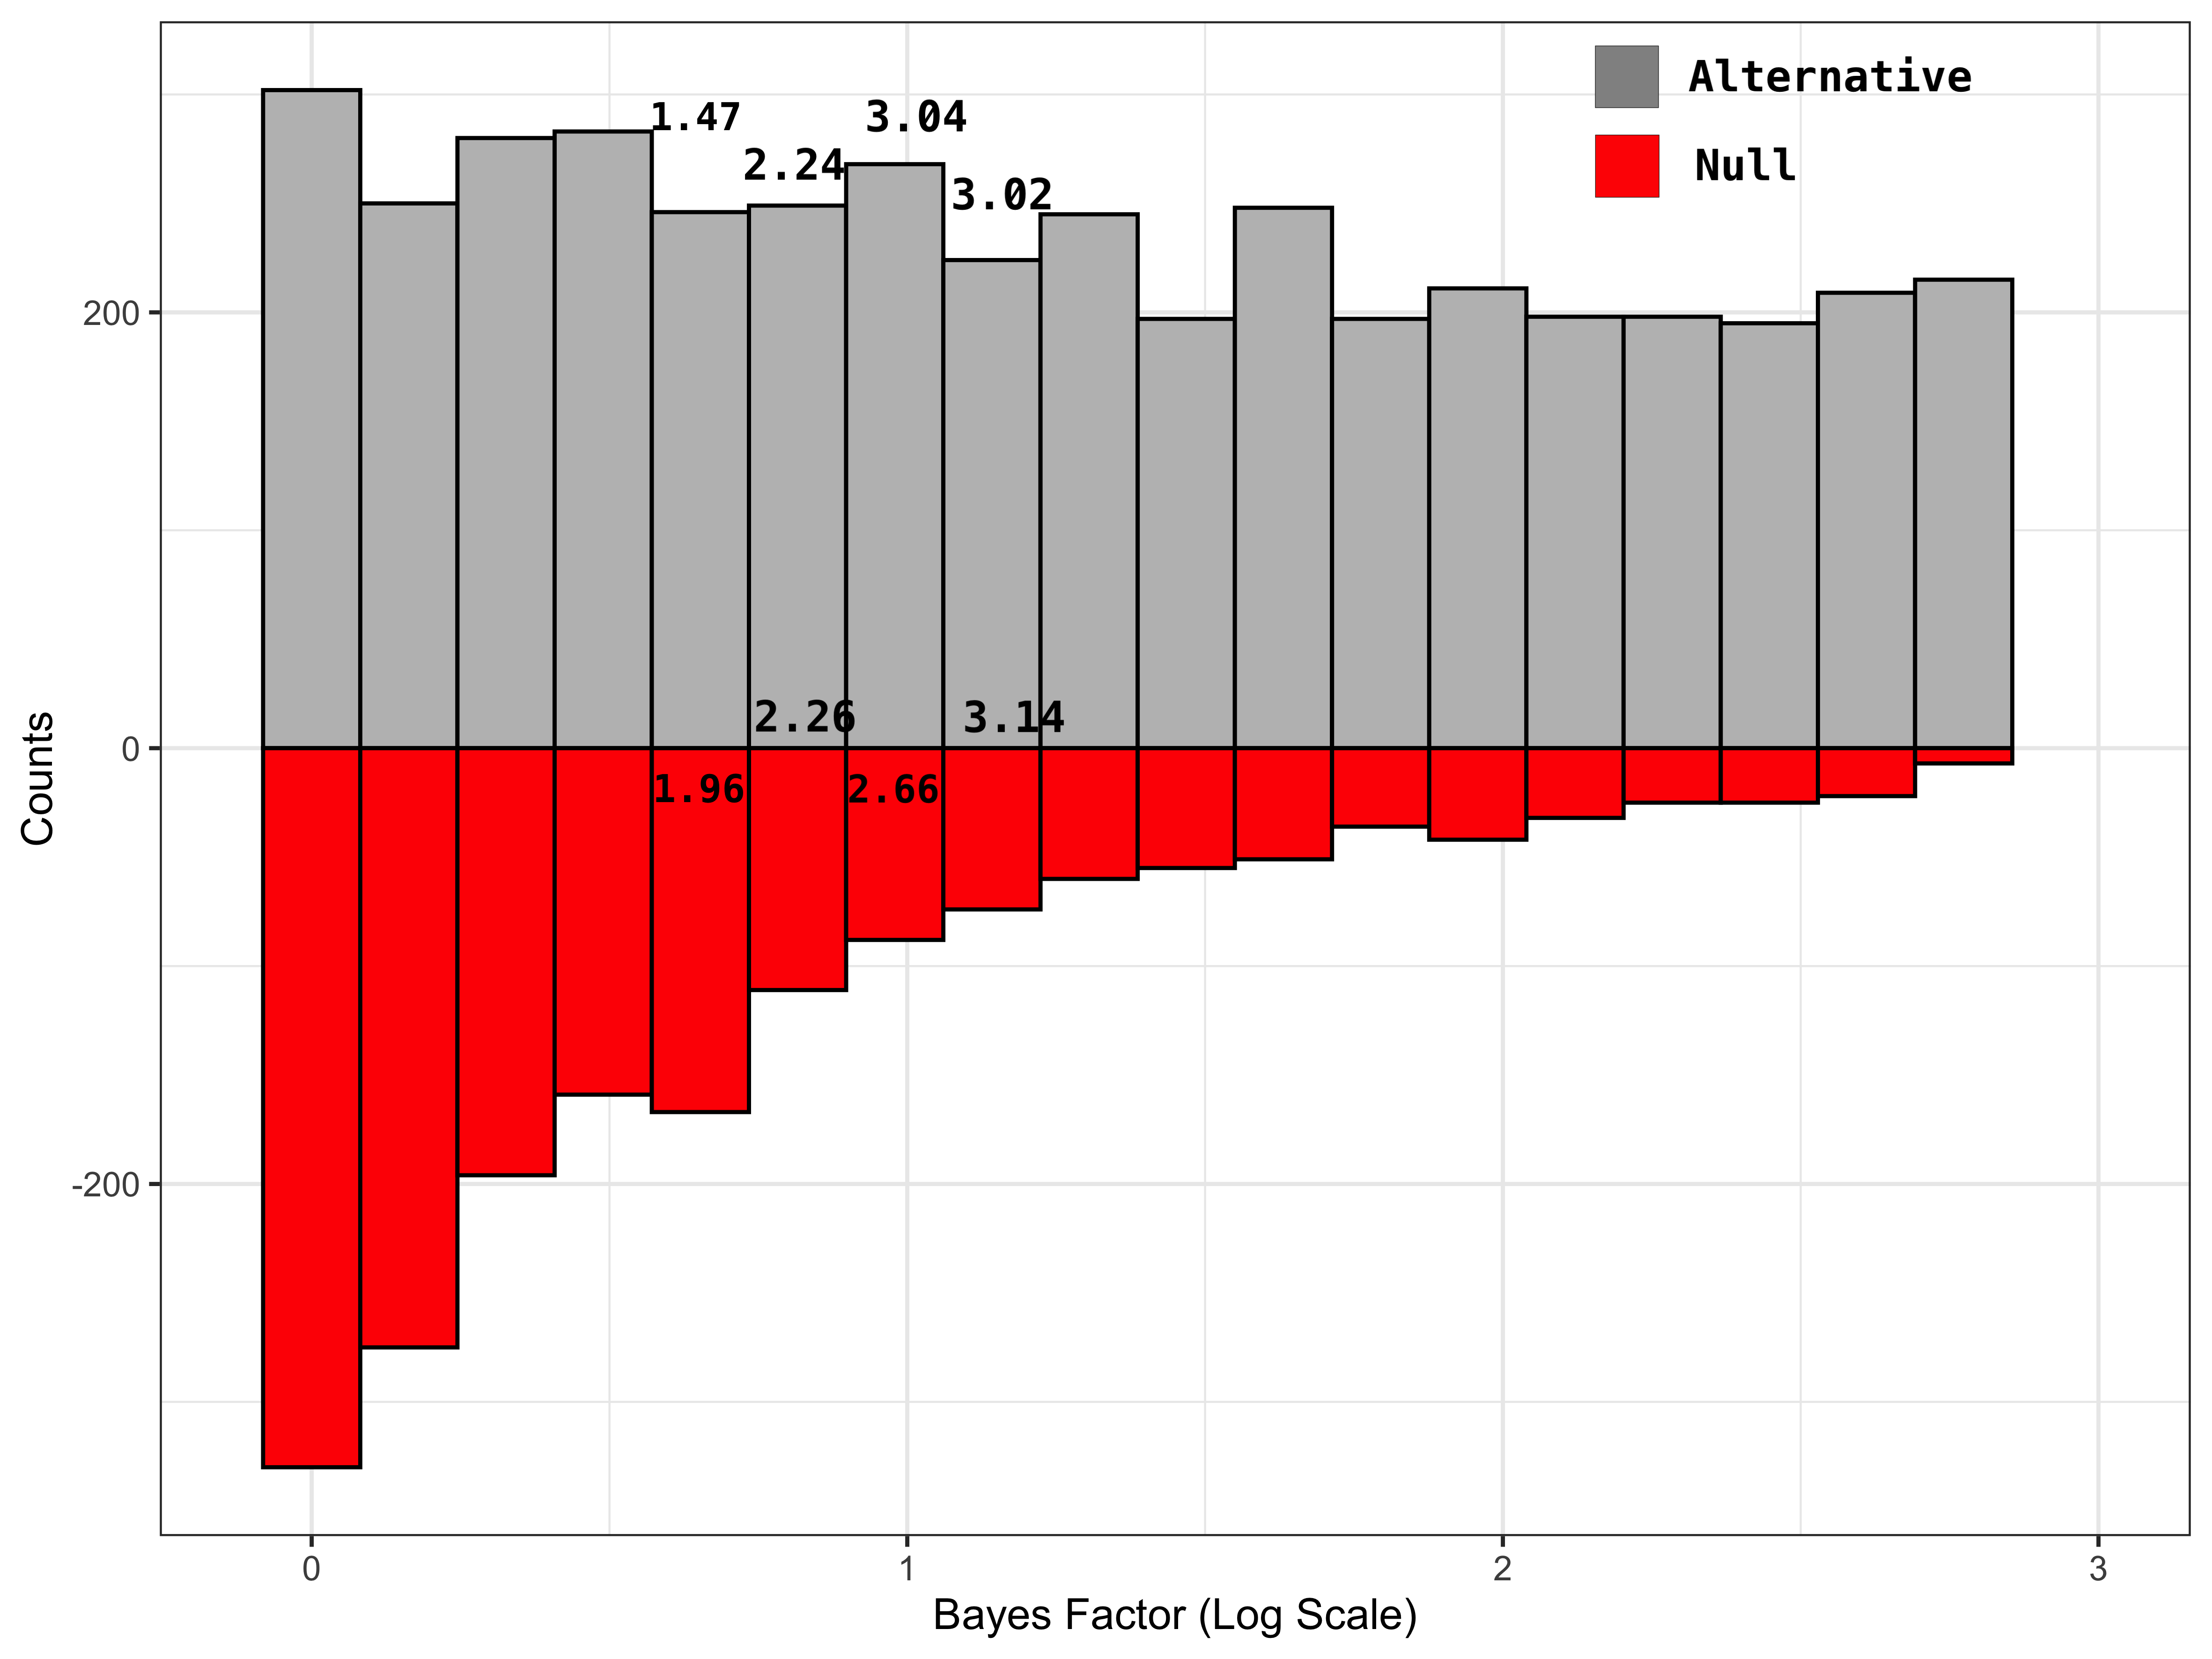
\includegraphics[width=.3\textwidth]{template-komputasi-latex/example1N.png}\hfill
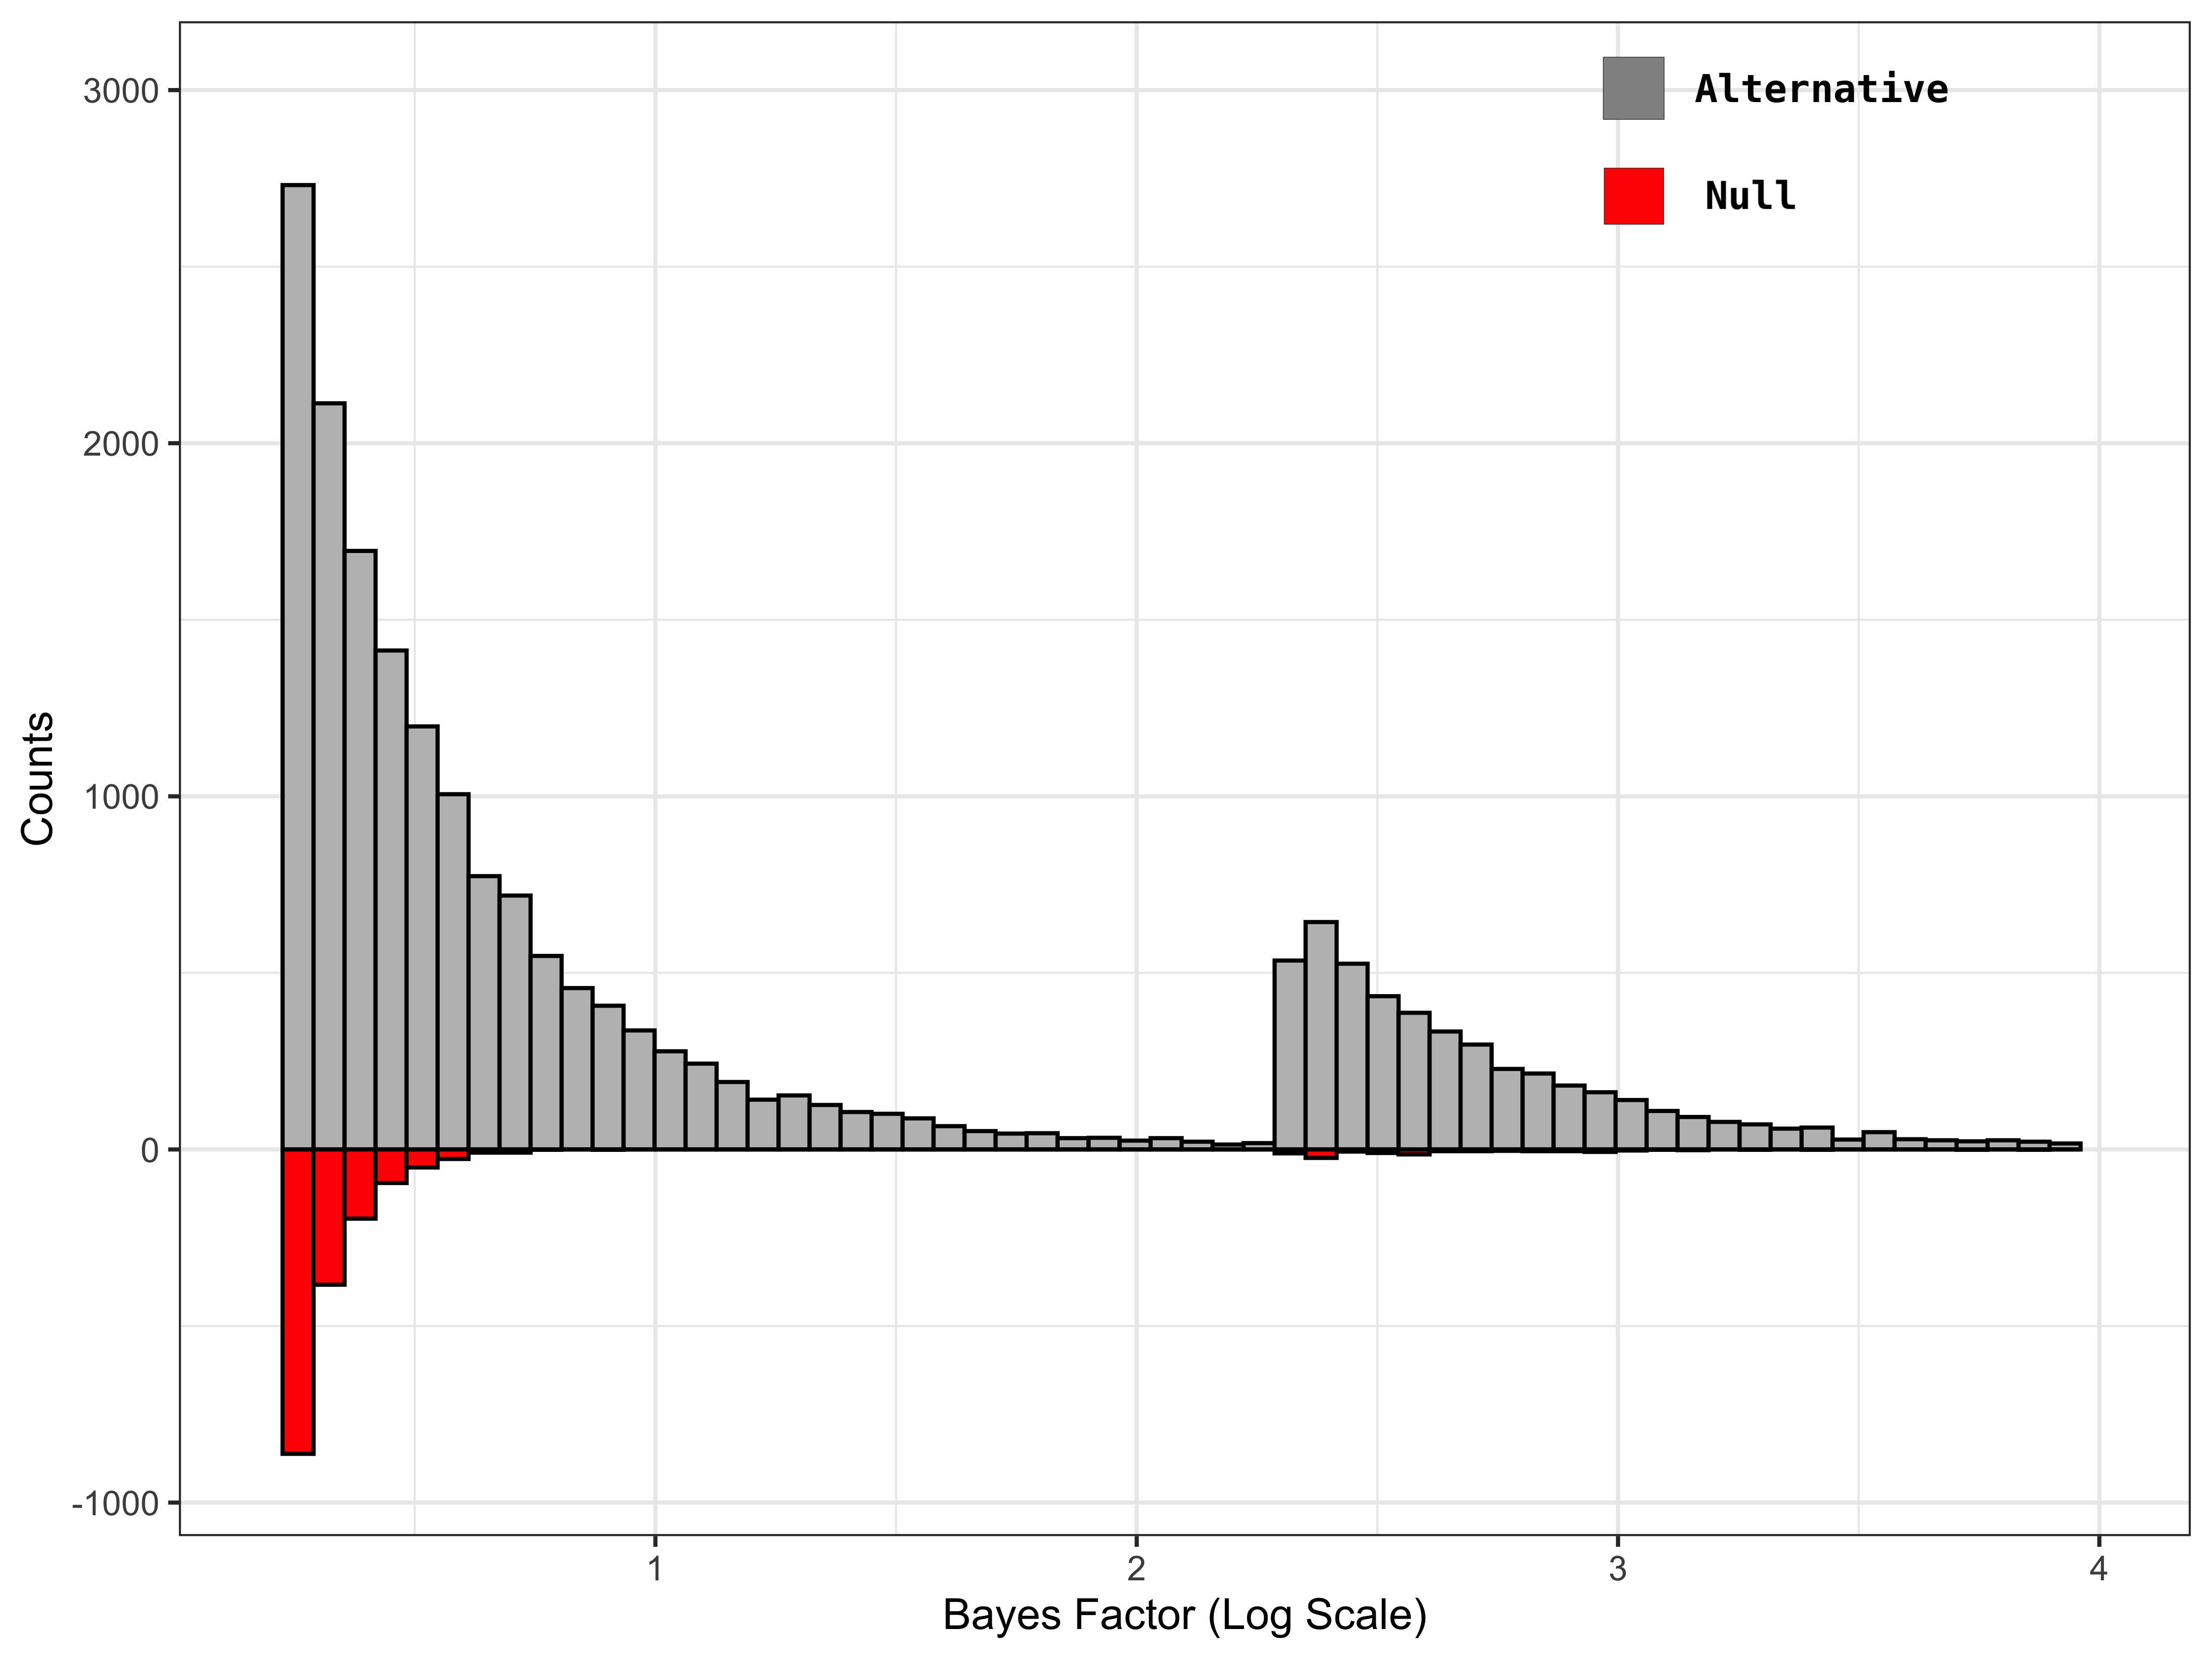
\includegraphics[width=.3\textwidth]{template-komputasi-latex/example_stopping.png}\hfill
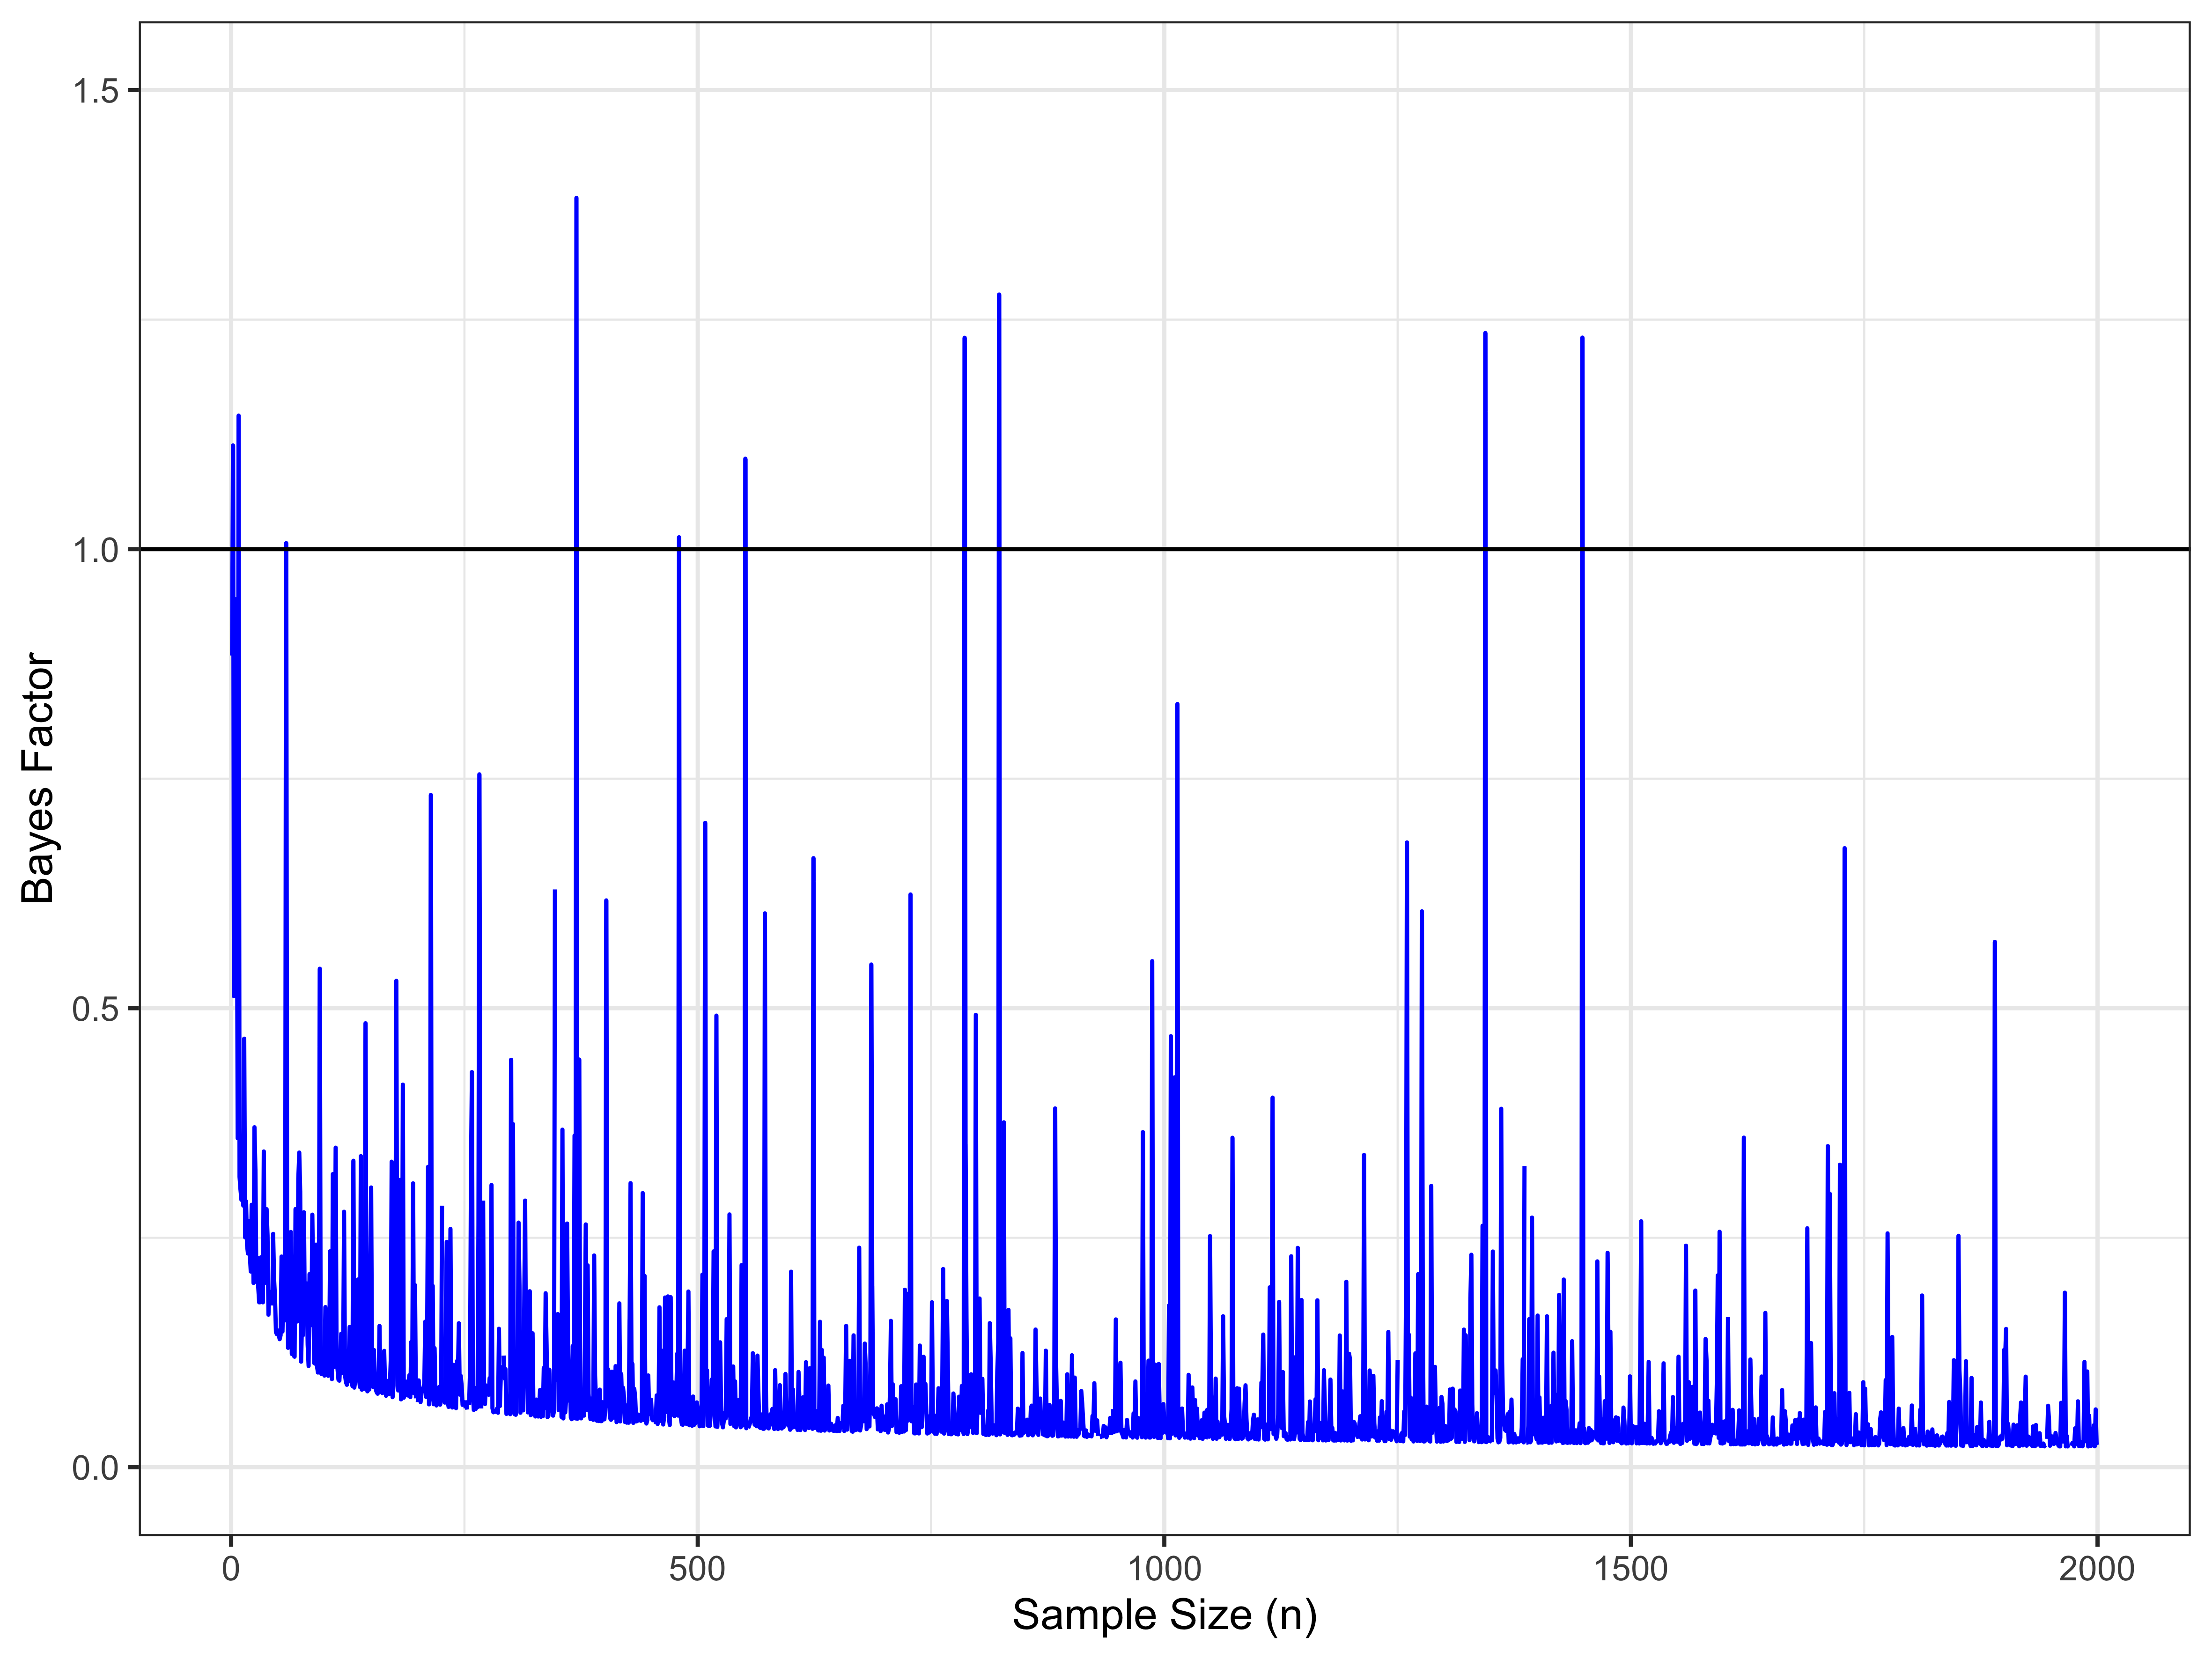
\includegraphics[width=.3\textwidth]{template-komputasi-latex/bayes_over_n.png}

\caption{(a) Estimated posterior odds stacked against the frequency of H1/H0 when sample size is fixed to N = 100. The numbers at the top represent the frequency odds and the numbers near the axis the posterior odds/Bayes factors (b) Estimated posterior odds stacked against the frequency of H1/H0 when optional stopping is implemented for bounds of 10 and 1/10 (c) Estimated Bayes factor over several sample sizes for one simulated dataset with data generated under $H_0$ for sample sizes from 1 to 2000. The colours represent which model the underlying data were generated from}
\label{fig:figure3}

\end{figure}

Overall, this plot provides quite an intuitive understanding of the posterior odds. By definition, looking at bin with Bayes factor 2.26:1 in favour of the alternative, we expect the alternative to be 2.26 times as probable to have produced the data \cite{rounder}. As we see here, this figure intuitively shows us this as there around 2.24 times more when the selected model was the alternative over the null in the 50,000 repetitions. Interestingly, we also see this property hold even though we arbitrarily stopped at the threshold K in Figure 1(b). as the bins generated under the two hypotheses still match up, although the shapes of the two distributions have changed. 

\section{Calibration of the Posterior Odds}

Figure 1(a) and 1(b) above essentially both express a calibration property of the posterior odds. Thus, under a stopping rule $K$ that has been defined apriori (even just the magnitude of reasonable effect that we are interested in seeing works), the interpretation of the posterior odds can still remain unbiased, even with optional stopping. Specifically, conditioned on data whose posterior odds equal to some $q$, we have: 
\begin{equation}
    \frac{\mathbb{P}(H_1|PostOdds = q)}{\mathbb{P}(H_0|PostOdds = q)} = q
\end{equation}

This calibration guarantees that the result of our test performed above remains the same in terms of interpretation of the posterior odds and Bayes factor even with continuous monitoring of the data till it has reached a certain effect size \cite{deng}. This holds provided that the posterior odds are calculated based on a defined stopping criteria $K$ with all data up until this point. Looking at Figure 1(c), where the Bayes factor is plotted over several sample sizes, for instance, although we notice the \textit{consistency} of the estimate with increasing sample size coverging to 0, we can also see that there are chances of inflated Type-I error still, particularly at large sample sizes (and additionally as our effect size is quite small). Thus for me to first generate this figure and then to say use only the subset of this dataset up until the spikes of the Bayes factor (to get a Bayes factor that shows evidence for the alternative, albeit very modest evidence) would likely violate this calibration. 

\section{Example 2: Model Misspecification in a one-sample hypothesis test for mean}

The computation of the Bayes factor (and the associated posterior odds) are both quite dependent on the specifications of the models being compared. Thus, it was of interest to me to see if the nice optional stopping properties we saw earlier still held under a case of model misspecification. To explore this, we go back to our one-sample hypothesis test setup but modify it so that we are no longer evaluating a composite hypothesis, but two directional point alternative hypotheses. We simulate gathering data $\textbf{D}$: $x_1....x_n$ from a normal distribution $\mathbb{N}(0, 1)$ (under the null point effect, a true effect size of 0) where we test for a moderate positive ($\delta_1 = 0.5$) and negative effect respectively ($\delta_2 = -0.5$) \cite{rounder, wage, hill}. Naturally, our model construction is misspecified here, as we are testing for two directional effects while the real data has been generated assuming a true zero effect \cite{wage}. The Bayes factor in this case can be represented as: 
\begin{equation}
\frac{\textnormal{exp}(-(\bar{X}-\delta_1))/(2/N)}{\textnormal{exp}(-(\bar{X}-\delta_1))/(2/N)}
\end{equation}
Here, we follow a slightly different simulation setup, wherein we sample from the null and then calculate the Bayes factor under 1) a fixed sample size of $N = 50$ and 2) under the same optional stopping criterion used in Example 1. Figure 2 shows the simulation results from this example. 

\begin{figure}[H]

\centering
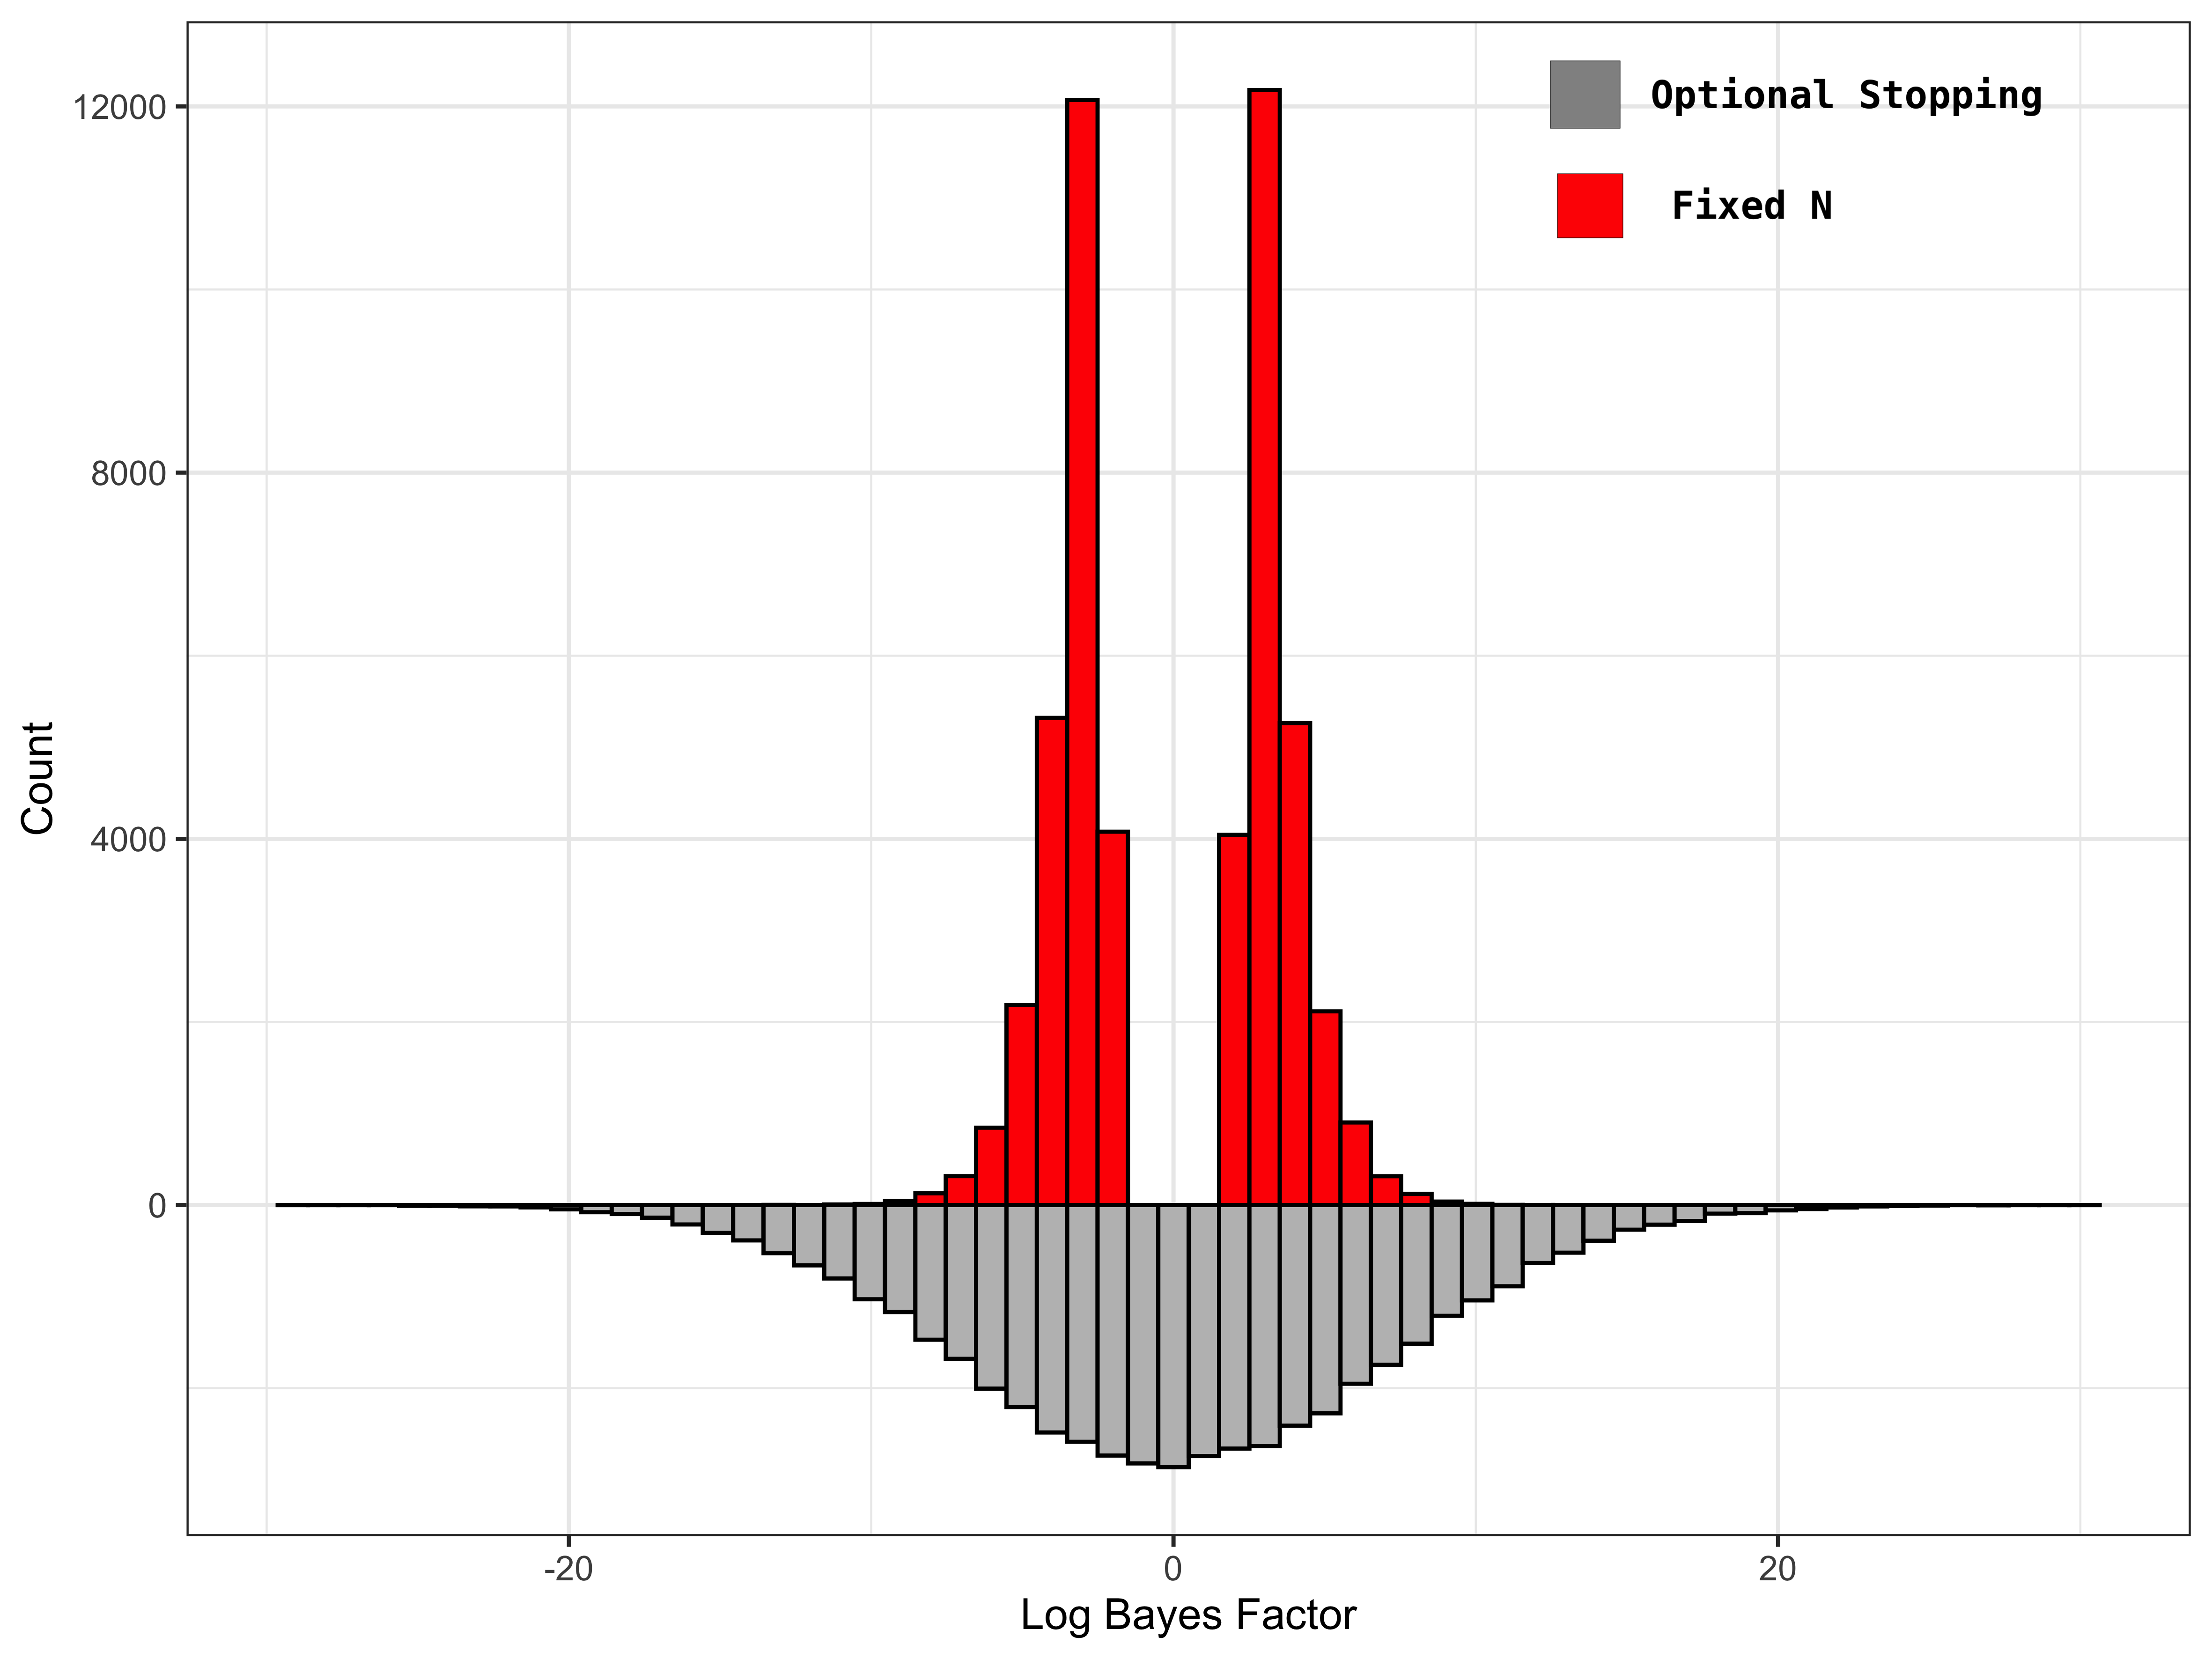
\includegraphics[width=.5\textwidth]{template-komputasi-latex/hist_opt.png}\hfill
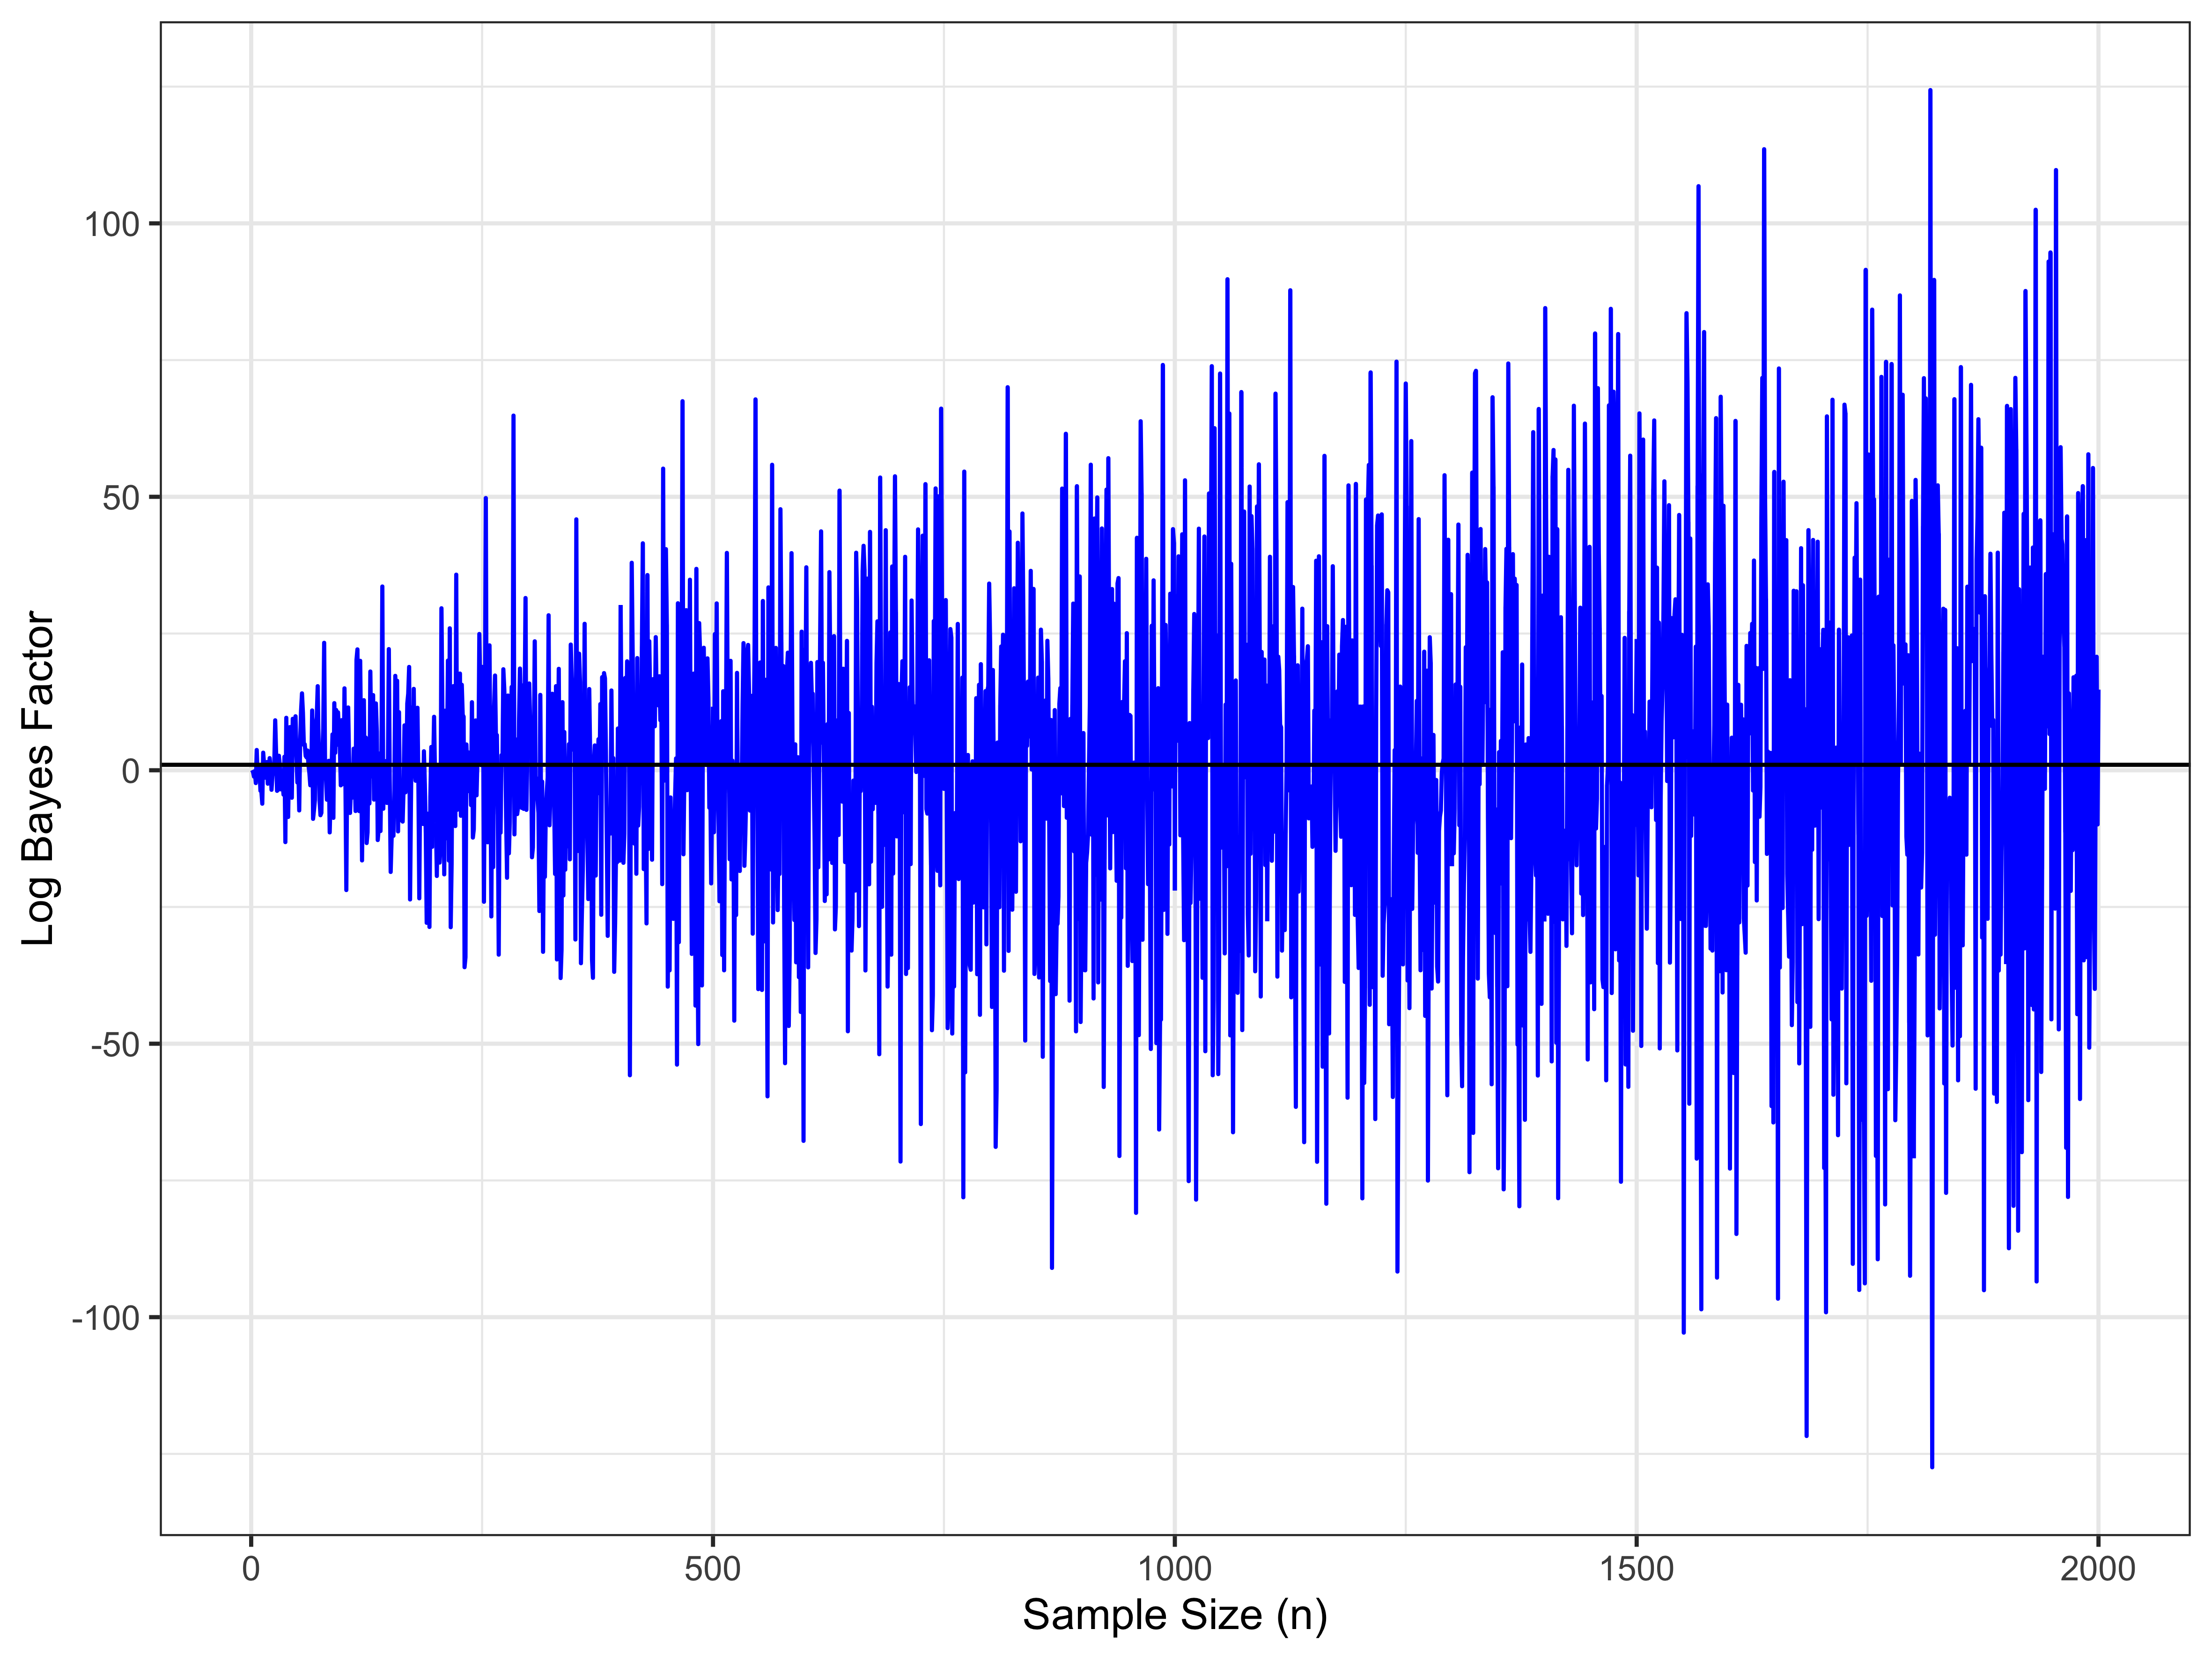
\includegraphics[width=.5\textwidth]{template-komputasi-latex/model_misspecification.png}\hfill

\caption{(a) Log transformed estimated posterior odds against the frequency of H1/H0 when sample size is fixed to N = 100. The red distribution is the posterior odds under optional stopping and the grey represents the fixed sample size analysis of N = 50  (b) Log transformed estimated Bayes factor over several sample sizes for one simulated dataset with data generated under $H_0$ with misspecified models for sample sizes from 1 to 2000}
\label{fig:figure3}

\end{figure}

In Figure 2(a), we notice that with optional stopping there is a greatly increased posterior odds (keep in mind this is on the log scale) of selecting one of the directional models (with slightly larger support for selecting the positive effect) and practically no odds of a Bayes factor around 1. This may not be surprising however, when we look at Figure (b), where we see essentially that under this model misspecification, the Bayes odds tend to meander randomly between support for the two hypotheses, with the increasing sample sizes rather than converging to 0 or Infinity, as p-values also tend to do under NHST \cite{wage}. Thus, we can infer that in this scenario the nice calibration properties of Bayes odds in relation to optional stopping do not apply, as a researcher can bide their time and be certain collect strong evidence for their favored direction even where there is no such effect \cite{wage}. 

We can note that this will definitely not be an issue had one of the comparison models been the null hypothesis \cite{wage}. Thus, some care must be exercised when specifying the models that are to be evaluated for the Bayesian model comparison to make sure that they are compatible with the data generation, and to pick models that are "worthy of our consideration". These results do not impinge on the general nice calibration property discussed earlier for well-specified models \cite{rounder}. It would also be interesting to consider the lecture model comparison example, where the true values were drawn from both models and look at the results of optional stopping. Finally another interesting model misspecification is prior misspecification which effects the Bayes factor and posterior odds generated. In particular, it would be interesting to explore if specifying a highly informative prior can give strong evidence for a favoured direction as well \cite{heid}. 

Overall, we have explored the calibration property of posterior odds under optional stopping in the Bayesian framework. While Bayesian model comparison is not an for-all-case panacea,  When performed \textit{properly} with a pre-defined stopping rule (i.e no double dipping, data subsetting or future forecasting) and when both the models under comparison are well-specified, valid inferences can certainly be made under optional stopping conditions with Bayesian model comparison, likely with smaller sample sizes, and to the end of observing reasonable effects.  

\section{Code}

Code used for simulations and for generating figures can be found here: \url{https://github.com/ntmv/optional-stop-misc}.
%\begin{figure}[h]
%	\centering
%	\includegraphics[width=0.5\textwidth]{images/figur1.PNG}
%	\caption{Font 10pt and center not bold for captions except for the words "Figure"}
%	\label{fig1}
%\end{figure}



%\subsection{Table (10pt, bold)}
%Writing tables are numbered followed by the title of the table above the table, centered, 1 spaced with a short and precise title. Consider the example in Table \ref{table1}
%\begin{table}[h]
%	\centering
%	\caption{Font 10pt and center not bold for captions except for %the words "Table"}
%	\label{table1}
%	\begin{tabular}{@{}cccc@{}}
%		\toprule
%		\textbf{Characteristics}& \textbf{Description }& \textbf{Frequency }& \textbf{Percentage} \\
%		\midrule
%		Gender & Male & 198 & 80.2\% \\
%		& Female & 49 & 19.8\% \\
	%	Entry & 2018 & 54 & 21.9\% \\
	%	& 2019 & 64 & 25.9\% \\
	%	& 2020 & 59 & 23.9\% \\
	%	& 2021 & 70 & 28.3\% \\
	%	MBKM & Yes & 217 & 87.9\% \\
	%	& No & 30 & 12.1\% \\
	%	& Total & 247 & 100\% \\
	%	\bottomrule
	%\end{tabular}
%\end{table}


%\subsection{Figure (10pt, bold)}
%Image writing techniques in scientific papers must also be symmetrical in the middle. So the settings are not aligned right or left, but in the center. This helps tidy up the position of the image or photo so that it appears side by side well with the description text as in Figure \ref{fig2}.

%\begin{figure}[h]
%	\centering
%	\includegraphics[width=0.5\textwidth]{images/figur2.PNG}
%	\caption{Font 10pt and center not bold for captions except for the words "Figure"  }
%	\label{fig2}
%\end{figure}


%\section{Result and Discussion (10pt, bold)}


\bibliographystyle{IEEEtran}

%\bibliography{template} %-->reference list is on the template.bib file
\begin{thebibliography}{1.7} 
	\bibitem[1]{rounder} \color{blue}R. J. N. Rouder, “Optional stopping: No problem for bayesians,” Psychonomic Bulletin &amp; Review, vol. 21, no. 2, pp. 301–308, 2014. \color{black}
	\bibitem[2]{deng} \color{blue}A. Deng, J. Lu, and S. Chen, “Continuous monitoring of A/B tests without pain: Optional stopping in Bayesian testing,” 2016 IEEE International Conference on Data Science and Advanced Analytics (DSAA) [Arxiv], 2016.  \color{black}
 \bibitem[3]{wage} \color{blue} E.-J. Wagenmakers, Q. F. Gronau, and J. Vandekerckhove, “Five bayesian intuitions for the stopping rule principle,” Arxiv, 2019.  \color{black}
 \bibitem[4]{heid} \color{blue} R. de Heide and P. D. Grünwald, “Why optional stopping can be a problem for Bayesians,” Psychonomic Bulletin &amp; Review, vol. 28, no. 3, pp. 795–812, 2020. \color{black}
 \bibitem[5]{hill} \color{blue} A. N. Sanborn and T. T. Hills, “The frequentist implications of optional stopping on Bayesian hypothesis tests,” Psychonomic Bulletin &amp; Review, vol. 21, no. 2, pp. 283–300, 2013. \color{black}
	
\end{thebibliography}


\end{document}